\newcommand{\xinf}{\underline{\vect{x}}}%
\newcommand{\xsup}{\overline{\vect{x}}}%
\newcommand{\xinit}{\vect{x}_0}%
\newcommand{\traj}{\varphi}%
\newcommand{\xn}{\vect{x}_n}%
\newcommand{\un}{\vect{u}_n}%
\newcommand{\wn}{\vect{w}_n}%
\newcommand{\yn}{\vect{y}_n}%
\newcommand{\xnn}{\vect{x}_{n+1}}%
%
\section{Reached sets computation}
%
The computation of the reached sets is a field in control theory on its own.
So the reader might refer to the large literature about this field for more precise algorithms in order to find invariants and the reached sets.

In this part, we will present 2 methods to compute the reached sets.
The first one will only be valid for monotone systems, even if this class is restrictive, it is possible to obtain a closed form solution for the problem which might be useful for further studies.
The second one is based on ellipsoidal bounding methods which can be applied to a wider class of systems. 


\subsection{Monotone systems}
Monotone systems are systems that keep a partial ordering relation between 2 trajectories. With this property, we can bound a set by 2 vectors $\xinf$ and $\xsup$.
For all the trajectories starting at $\xinit \in [\xinf,\xsup]$, we know that
\begin{equation}
\forall k \in \mathbb{N}, \traj(\xinit,k) \in [\traj(\xinf,k),\traj(\xsup,k)]
\end{equation}

We will work with a linear monotone system defined by:
\begin{equation} \label{sys:monotone_lti}
\begin{split}
\xnn &= A \xn + B \un + E \wn \\
\yn &= C \xn
\end{split}
\end{equation}

\cite{liu2014abstraction} have been investigating boundedness property in order ignore one part of the abstraction.
Really good introduction about hierarchical control approach, give references.

Let define the system $S$

\begin{align*}
\mathbf{x}_{n+1} &= 
\begin{bmatrix} A_z & A_{zr}\\ 0 & A_r \end{bmatrix} \mathbf{x}
+\begin{bmatrix} B_z \\ B_r \end{bmatrix} \mathbf{u}
+\begin{bmatrix} E_z\\ E_r \end{bmatrix}\mathbf{w}\\
\mathbf{y}_n &= \mathbf{x}^z_n
\end{align*}
with,
\begin{align*}
\mathbf{x}_n = \begin{bmatrix}
\mathbf{x}^z_n\\
\mathbf{x}^r_n
\end{bmatrix}
\textrm{, }
\mathbf{u} = \begin{bmatrix}
\mathbf{u}^z_n\\
\mathbf{u}^r_n
\end{bmatrix}
\textrm{, }
\mathbf{w}_n = \begin{bmatrix}
\mathbf{w}^z_n\\
\mathbf{w}^r_n
\end{bmatrix}
\end{align*}

Let $S_r=(A_r,B_r,E_r)$ the subsystem of $S$, $\mathcal{U}_r$ and $\mathcal{W}_r$ the projection of $\mathcal{U}$ and $\mathcal{W}$ on the reduced system input space and noise space respectively.

We will assume the subsystem $S_r$ is a monotone stable system and that the inputs and noise are bounded.
These hypotheses might seems really restrictive, however most of the control strategy consist of stabilizing one part of the system that might be independent of the rest of the system.
Further analysis will show that if the controlled part of the system is as reactive as the abstraction sampling time, this reduction might lead to good results.

We would like to find all the reachable states of $S_r$.
Let $|\lambda_1| \leq ... \leq |\lambda_{n_r}|$ the eigenvalues of $A_r$, as the system $S_r$ is asymptotically stable $|\lambda_{n_r}|<1$,
so the eigenvalues of the matrix $I-A_r$ are all greater than 0.
Let define:
\begin{equation}
\begin{split}
\overline{\mathbf{x}}^r &= (I-A_r)^{-1} (B_r \overline{\mathbf{u}}^r + E_r \overline{\mathbf{w}}^r)\\
\underline{\mathbf{x}}^r &= (I-A_r)^{-1} (B_r \underline{\mathbf{u}}^r + E_r \underline{\mathbf{w}}^r)\\
\end{split}
\end{equation}

where $\mathcal{U}^r \subset \left [\underline{\mathbf{u}}^r, \overline{\mathbf{u}}^r \right ]$ and $\mathcal{W}^r \subset \left [\underline{\mathbf{w}}^r, \overline{\mathbf{w}}^r \right ]$, such bounds exists as we assumed that $\mathcal{U}_r$ and $\mathcal{W}_r$ are bounded.

Let $\varphi_r (\mathbf{x}^r,U_r,W_r)$ the trajectory function of the system $S_r$ starting from $\mathbf{x}^r$
applying the control sequence $U_r \in \mathcal{U}_r^\star$
with the noise sequence $W_r \in \mathcal{W}_r^\star$.
As the system $S_r$ is monotone,
$$
\forall \mathbf{x}^r \in \left [\underline{\mathbf{x}}^r, \overline{\mathbf{x}}^r \right ],
\forall U_r \in \mathcal{U}_r^\star,
\forall W_r \in \mathcal{W}_r^\star,
\varphi_r(\mathbf{x}^r,U_r^e,W_r)
\in \left [\underline{\mathbf{x}}^r, \overline{\mathbf{x}}^r \right ]$$

If the initial state of the reduced system is in $\left [\underline{\mathbf{x}}^r, \overline{\mathbf{x}}^r \right ]$, then every trajectories will stay in this set.

For $U_r \in \mathcal{U}_r^\star$, let $X_r(U_r)$ the subset of $\mathbb{R}^r$ defined by:
\begin{equation}
X_r(U_r) = \left [ 
\varphi_r(\underline{\mathbf{x}}^r,U_r,\underline{\mathbf{w}}^r),
\varphi_r(\overline{\mathbf{x}}^r,U_r,\overline{\mathbf{w}}^r)
\right ]
\end{equation}
$X_r(U_r)$ correspond to the set of all the possible successors after applying the control sequence $U_r$ on the system $S_r$. This results come from the monotonic property.
This can be summarized in the following property:
$$
\forall U_r \in \mathcal{U}_r^\star,
\forall \mathbf{x}^r \in \left [\underline{\mathbf{x}}^r, \overline{\mathbf{x}}^r \right ],
\forall W_r \in \mathcal{W}_r^\star,
\varphi_r(\mathbf{x}^r,U_r,W_r)
\in X(U_r)$$

\subsection{Extension to non monotonic systems}
The main argument behind the reduction is the ability to bound the dynamic in a set and to work with these boundaries (which are easier to manipulate than a complete system).
The monotonicity property is really convenient in order to perform the computations.
However, this is a strong assumption on the system that cannot be met in every situations: any system that have a non real eigenvalues is not monotonic.
In this part we will have a Lyapunov approach for a linear system.
The Lyapunov function will not be used to proof the stability of the system but to perform operations on bounding sets of our dynamic.

The natural representation of bounds with the monotonicity property are rectangle, in our case, the lyapunov function that we will use is a quadratic function $\vect{x}^T P \vect{x}$ where $P$ is a definite positive matrix.
Even if the lyapunov approach is usable for a monotonic, we will see that it is less efficient than the monotonic approach.

To perform the reduction, we have to find the best combination of applying the reduction: the different theory must be used in a proper way. The monotonicity property depends on the base of the system. The lyapunov function efficiency also depend on the frame.

Lets consider the previous linear system.
Lets denote $x^\star(u,w)$ the equilibrium point of the linear system, the previous assumptions about global stability will still hold:
\begin{equation}
\vect{x}^\star(\vect{u},\vect{w}) = A^{-1} (B \vect{u} + E \vect{w})
\end{equation}

\begin{equation}
\vect{x}^{\star}_{\vect{u}} = \vect{x}^\star(\vect{u},\vect{0})
\end{equation}

Lets define the following Lyapunov function obtained by solving the Lyapunov equation $A^T P + P A = -Q$ where $Q$ and $P$ are positive definite ($Q$ is given):

\newcommand{\xu}{\vect{x}^{\star}_{\vect{u}}}
\newcommand{\Vu}{V_{\vect{u}}}
\begin{equation}
\Vu(\vect{x}) = (\vect{x} - \xu) ^T P (\vect{x} - \xu) 
\end{equation}

In the next paragraphs, we will try to find invariant sets:
\begin{align*}
\dot{\Vu}(t) =& \dot{\vect{x}}^T(t) P (\vect{x}(t) - \xu) +  (\vect{x}(t) - \xu)^T P \dot{\vect{x}}(t)
\\
 =& (A \vect{x}(t) + B \vect{u} + E \vect{w}(t))^T P (\vect{x}(t) - \xu)\\
 & + (\vect{x}(t) - \xu)^T P (A \vect{x}(t) + B \vect{u} + E \vect{w}(t))
\\
 =& (A (\vect{x}(t) - \xu) + E \vect{w}(t))^T P (\vect{x}(t) - \xu)\\
 & +(\vect{x}(t) - \xu)^T P (A (\vect{x}(t) - \xu)+ E \vect{w}(t))
\\
 =& (\vect{x}(t) - \xu)^T A^T P (\vect{x}(t) - \xu) +  (\vect{x}(t) - \xu)^T P A (\vect{x}(t) - \xu)\\
 & + (E \vect{w}(t))^T P (\vect{x}(t) - \xu) +  (\vect{x}(t) - \xu)^T P E \vect{w}(t)
\\
 =& - (\vect{x}(t) - \xu)^T Q (\vect{x}(t) - \xu)\\
 & +\vect{w}(t)^T E^T P (\vect{x}(t) - \xu) +  (\vect{x}(t) - \xu)^T P E \vect{w}(t)\\
\end{align*}

Please note the following inequality:
\begin{equation}
- (\vect{x}(t) - \xu)^T Q (\vect{x}(t) - \xu) \leq - \alpha \Vu
\end{equation}

where
\begin{equation}
\alpha = \frac{\lambda_{min}(Q)}{\lambda_{max}(P)}
\end{equation}
Thanks to the positive definite property of $Q$ and $P$, we have $\alpha>0$.

In the next part we will try to find an upper bound for $(\vect{x}(t) - \xu)^T P E \vect{w}(t)$ and $(E \vect{w}(t))^T P (\vect{x}(t) - \xu)$.

We want to solve the following problem:
\begin{equation} \label{eq:max_w}
\max_{\vect{w} \in \mathcal{W}} \vect{b}^T \vect{w}
\end{equation}
In order to simplify the problem, we will take $\mathcal{W} = \{ \vect{w} \in \mathbb{R}^q \mid \vect{w}^T R \vect{w} \leq S\}$ where $R$ is a (strictly) positive definite matrix and $S>0$ a real number that correspond to the noise magnitude.
By writing the Lagrange multiplier, we can find that the maximum of this function is reached when:
\begin{equation}
\tilde{\vect{w}} = \frac{S^{\nicefrac{1}{2}} R^{-1} \vect{b}}{(\vect{b}^T R^{-1} \vect{b})^{\nicefrac{1}{2}}}
\end{equation}
\textit{Carefull there, it is not always defined!!!}

The maximum of $(\vect{x} - \xu)^T P E \vect{w}$ for a given $\vect{x}$ and $\xu$ is:
\newcommand{\Vwu}{V_{\vect{u}}^{\mathcal{W}}}
\textit{This result is false, it must be something like $P E^T R E P^T $}
\begin{equation}
\Vwu(\vect{x}) = [S (\vect{x} -\xu)^T E^T P R P^T E (\vect{x} -\xu)^T ]^{\nicefrac{1}{2}}
\end{equation}
\textit{I need to compute the actual value of $\beta$}
Let $K = E^T P R P^T E$
We will assume that $K$is defined positive.
This hypothesis is not too strong, $R$ has been chosen positive definite.
$P$ is already chosen to be positive definite.
So $E$ needs to be positive definite so that $K$ is positive definite.

For all $\vect{x} \in \mathcal{X}$, let $\vect{y} = \vect{x} -\xu$:
$$\vect{y}^T K \vect{y} \leq  \lambda_{max}(K) \vect{y}^T \vect{y}$$
As $P>0$, $\lambda_{min}(P)>0$:
$$\vect{y}^T \vect{y} \leq \frac{1}{\lambda_{min}(P)}  \vect{y}^T P \vect{y}$$
We have $\Vu(\vect{y}) = \vect{y}^T P \vect{y}$, so:
$$\vect{y}^T K \vect{y} \leq \frac{\lambda_{max}(K)}{\lambda_{min}(P)}  \Vu(\vect{y})$$
\newcommand{\Bu}{\beta}
We will define $\Bu$ by:
$$\Bu = 2\sqrt{S \frac{\lambda_{max}(K)}{\lambda_{min}(P)} }$$

\begin{equation}
\Vwu(\vect{x}) < \frac{\Bu}{2} [\Vu(\vect{x})]^{\nicefrac{1}{2}}
\end{equation}
where $\Bu$ is computed with eigenvalues of $E$, $P$, and $R$.

From now we have the following inequality:
\begin{equation}
\dot{\Vu}(t) \leq -\alpha \Vu(t) + \Bu \Vu^{\nicefrac{1}{2}}(t)
\end{equation}

Please note that this inequality is "optimal" in the sense that the upper boundary is reached when  we choose $\vect{w}$ solution of the maximization problem \ref{eq:max_w}.

\begin{prop} \label{ineq:lyap}
The function $\Vu$ verify this inequality for all $t',t \in \mathbb{R}^+$, with $t'>t$:
\begin{equation}
\Vu(t') \leq  \left[ (\sqrt{\Vu(t)} - \frac{\Bu}{\alpha}) e^{-\frac{\alpha}{2} (t'-t)} + \frac{\Bu}{\alpha} \right] ^2
\end{equation} 
\end{prop}

\begin{proof}
\newcommand{\tI}{\underline{I}}
\newcommand{\tIs}{\overline{I}}
\textit{Choose another name for $u$, $u$ must just be the system input.}
For a trajectory $\vect{x}(t)$, the function $\Vu(t)$ is a continuous piecewise differentiable function as it can be expressed as the integral of a piecewise continuous function.
So we will limit the proof to this class of functions.

Let $u$ a continuous piecewise differentiable function that verify:
\begin{align*}
\dot{u} &\leq -\alpha u + \beta u^{\nicefrac{1}{2}}\\
u & \geq 0
\end{align*}
Let $I$ an interval of $\mathbb{R}^+$ (possibly unbounded).
If $\forall t\in I, u(t)=0$, as $\beta,\alpha>0$ the property is proved.
Let $I^0$ the interior of $I$.
Lets choose $I$ so that u is strictly positive and differentiable on $I^0$.
Let $f$ a function defined in $I^0$ by $f = \sqrt{u}$.
We have:
$$\dot{f} = \frac{\dot{u}}{2\sqrt{u}}$$
using the inequality, we get (in $I^0$):
$$\dot{f} \leq -\frac{\alpha}{2} f + \frac{\beta}{2}$$
Let $g = f- \nicefrac{\beta}{\alpha}$ (defined on $I^0$), 
by definition of $f$, $g$ is continuous and differentiable over $I^0$.
$$\dot{g} \leq -\frac{\alpha}{2} g$$
We can use the Gr\"onwall inequality for $t \in I^0$:
$$g(t) \leq g(0) e^{-\frac{\alpha}{2} (t-\tI)}$$
this imply that:
$$f(t) \leq (f(\tI)- \frac{\beta}{\alpha}) e^{-\frac{\alpha}{2} (t-\tI)} + \frac{\beta}{\alpha}$$
as $u \geq 0$ we have:
$$ u(t) \leq  \left[ (\sqrt{u(\tI)} - \frac{\beta}{\alpha}) e^{-\frac{\alpha}{2} (t-\tI)} + \frac{\beta}{\alpha} \right] ^2$$
We need now to prove this for all $t \in \mathbb{R}$.
Let the function $h$:
$$h(x,t) = \left[ (\sqrt{x} - \frac{\beta}{\alpha}) e^{-\frac{\alpha}{2}t} + \frac{\beta}{\alpha} \right] ^2$$
This function verify
\begin{equation} \label{eq:h_compo}
h(h(x,t_1),t_2) = h(x,t_1+t_2)
\end{equation}
Moreover:
\begin{equation} \label{eq:h_monot}
x \leq y \Rightarrow h(x,t) \leq h(y,t)
\end{equation}

For 2 consecutive interval $I_1$ and $I_2$ (so that $\tIs_1 = \tI_2$) of $\mathbb{R}^+$, and $t \in I_1$, we have:
$$u(t) \leq  h(u(\tI_1),t-\tI_1)$$
and for $t \in I_2$:
$$u(t) \leq  h(u(\tI_2),t-\tI_2)$$
As $u$ is continuous, we have:
$$u(\tI_2) = u(\tIs_1)$$
so
$$u(\tI_2) \leq h(u(\tI_1),\tIs_1-\tI_1)$$
which give for $t \in I_2$:
\begin{align*}
u(t) &\leq h(u(t),t-\tI_2) \\
&\leq h(h(u(\tI_1),\tIs_1-\tI_1), t - \tI_2) && \text{eq. \ref{eq:h_monot}}\\
&\leq h(h(u(\tI_1),\tIs_2-\tI_1), t - \tI_2) && \text{as $\tIs_1=\tI_2$}\\
& \leq h(u(\tI_1), t - \tI_1) && \text{eq. \ref{eq:h_compo} }
\end{align*}
So we proved that the property valid over $I_1$ is also valid over $I_2$.
We can apply successively this property over all intervals where $u$ is continuous and differentiable, this give us the following result:
$$u(t) \leq h(u(0),t)$$
which prove the property.
\end{proof}

Possible trajectories of the energy function:


\newcommand{\Vub}{\mathcal{V}_{\vect{u}}}
Let $\Vub$ the function defined by:
$$\Vub(t,\vect{x}) =  \left[ (\sqrt{\Vu(\vect{x})} - \frac{\beta}{\alpha}) e^{-\frac{\alpha}{2} t} + \frac{\beta}{\alpha} \right] ^2$$

This correspond to the decrease of the Lyapunov function after $t$ starting from $\vect{x}$.

\newcommand{\Xu}{\mathcal{X}_{\vect{u}}}
We will also define the function $\Xu$:
\begin{equation}
\begin{array}{llll}
\Xu:& \mathbb{R}^+ 	&\rightarrow 	& 2^X\\
	& v 				& 				& \{\vect{x} \in X \mid \Vu(\vect{x}) \leq v\}
\end{array}
\end{equation}
The $\Xu(v)$ for $v\geq0$ set correspond to the set of all the states that have less than $v$ of energy.


\begin{prop}
For every trajectory of the system, we have:
$$\forall t'>t,\vect{x}(t') \in \{\vect{x} \in \mathbb{R}^n \mid \Vu(\vect{x}) \leq \mathcal{V}_u(t'-t,\vect{x}(t))\}$$
\end{prop}

\begin{proof}
Lets take trajectory with constant input $\vect{u}$ so that it exist a $t'>t$:
$$\Vu(\vect{x}(t'))>\mathcal{V}_u(t'-t,\vect{x}(t))$$
This violate the property \ref{ineq:lyap}.
\end{proof}

We will formulate the previous property with sets (this what we will use in order to build the reduction).
Lets define $\mathcal{X}_{\vect{u}}(Y,t)$ the set of all the successors of the set $Y$ applying the constant input $\vect{u}$.

$$\mathcal{X}_{\vect{u}}(Y,t) = \{x \in X \mid \Vu(\vect{x}) \leq \sup_{\vect{y} \in Y}(\Vu(\vect{y},t)) \}$$

\textit{I need to have look at uniformly ultimately bounded function. Keywords: Boundedness, Ultimate Boundedness, nonautonomous systems}

\textit{Also, I have to proof the invariance property. Try to have more uniform notation between the 2 proof, eventually try to get 1 formulation for the 12 of them.}

\textit{I can define the lyapunov function so that it is usable with Lasalle's theorem.}

\textit{Do a part about rectangles to ellipse and ellipse to rectangle.}

\textit{Do a paragraph about how to apply this theory, how eventually to mix the 2 of the theory in order to get the most of it.}

We need first to find the set of all the possible states.
This will be done by using exactly the same steps than before but considering that the input is unknown (in our case, this is the same than considering the input as a noise).

To do this, we are going to assume that all the inputs verify $\vect{u} G \vect{u} < F$ where $G$ is a positive-defined matrix and $F>0$ is a real.

Then by using the same maximization than before, we have :
\newcommand{\Vw}{V_{\mathcal{U}}^{\mathcal{W}}}
\newcommand{\Vsup}{\overline{V}}
\begin{equation}\label{eq:Vw}
\Vw(\vect{x}) =
[S (\vect{x})^T E^T P R P^T E \vect{x} ]^{\nicefrac{1}{2}}+
[F (\vect{x})^T B^T P G P^T B \vect{x} ]^{\nicefrac{1}{2}}
\end{equation}
As we did before, we will assume that the matrix $L = B^T P G P^T B$ is positive definite.
Also, let $\gamma$ the following quantity:
$$\gamma = 2 \sqrt{\frac{\lambda_{max}(L)}{\lambda_{min}(P)}} + \Bu$$

Using this one within \ref{eq:Vw}:
$$\Vw(\vect{x}) \leq \gamma [V(\vect{x})]^{\nicefrac{1}{2}}$$

This will affect the Lyapunov function inequality in the following way:
$$\dot{V}(t) \leq -\alpha V(t) + \gamma V^{\nicefrac{1}{2}}(t)$$

The same remark hold for this inequality as well, by choosing the right $\vect{u}$ and the right $\vect{w}$, this equality is an inequality.

This let us define the invariant set of of the system.


In the next parts, we are going extend the previous reduction thanks to the Lyapunov function that we are using.
\begin{prop}
The set $\mathcal{X}$ defined by:
$\mathcal{X} = \{x \in X \mid \Vw(\vect{x}) \leq \Vsup \}$
where 
$$\Vsup = \left[ \frac{\gamma}{\alpha} \right]^2$$
is an invariant set of the system \ref{eq:lin_sys}.
\end{prop}

\begin{proof}
\textit{I need to be more precise.}
This property comes from the Lasalle's invariance principle.
In order to use it, we will create the following function:
\newcommand{\Vt}{\tilde{V}}
\begin{equation}
\Vt(\vect{x}) =
\left \{
\begin{array}{ll}
V(\vect{x})-\Vsup& \textrm{if $V(\vect{x}) \geq \Vsup$}\\
0 & \textrm{otherwise}
\end{array}
\right.
\end{equation}
The function $\Vt$ is always positive.
We know that for any trajectory and for all $t \in \mathbb{R}^+$:
$$\dot{\Vt}(t) \leq 0$$
Thanks to the Lasalle's invariant principle, we know that all the state are converging in an invariant set $\mathcal{X}_i \subseteq \{ \vect{x} \in X \mid \dot{\Vt}(\vect{x})=0 \}$.
This prove the property.
\end{proof}

\begin{figure}
	\center
	\includestandalone[width=\textwidth]{lyap_plot}
	\caption{Example of system that converge to the set $\mathcal{X}$.}
\end{figure}

\subsection{Minimal set}
The less successors the a abstraction is creating the better it is.
This statement can give us some insight about how to choose the Lyapunov function.
We would like to solve the following problem:
\begin{equation}
\min Vol(\mathcal{X}(\Delta t, \left[u_{-n},\dots,u_{-1} \right] ))
\end{equation}
We will reduce the optimization problem to the previous work made on the Lyapunov functions.

This optimization problem is complex.
The fact that the lyapunov decay function is not a cionvex function in term of $\alpha$, $\gamma$ and $V0$. This disallow us from solving efficently with any algorithm.


\textit{Verify that when we do it with a discrete model, nothing get better}.
Using Linear Matrix Inequality can be a good approach for this problem.
Several optimization formulations are possible:
\begin{itemize}
\item maximizing the decay rate of the Lyapunov function ($\alpha$),
\item minimizing the size of the invarient sets ($\gamma$,$V_0$).
\end{itemize}
A combination of both might be possible.
However, we will concentrate on minimizing the size of the invariants.
Please note that the differences will mainly depend on the system.

\cite{Polyak200815349}
\cite{LMI_book}


\subsection{Lyapunov system reduction}
In the next parts, we will only work with discrete systems. For a given sampling rate $\Delta t$, we use the following notation:
$$\mathcal{X}(Y) = \mathcal{X}(Y,\Delta t)$$
$$\mathcal{X}_{\vect{u}}(Y) = \mathcal{X}_{\vect{u}}(Y,\Delta t)$$


\subsection{Monotonic and Lyapunov system reduction}
\paragraph{Rectangular to ellipsoidal and ellipsoidal to rectangular constraints transformations}:
The fact that we are working with 2 different kind of system (monotonic and asymptotically stable non monotonic systems) needs to converts constraints expressed in monotonic formulation to be expressed as constraints on norms.


\begin{figure}
	\center
	\includestandalone[width=0.7\textwidth]{monotone_to_ellipse}
	\caption{Figure of the ellipse to monotonic constraint (in blue) and the monotonic to ellipsoidal constraint (red).}
\end{figure}

\subsection{Reduction}
We have now a the same notation for stable monotonic and stable non monotonic systems plus a way of converting constraint of a non monotonic system to a monotonic system. We will now detail how to perform the reduction in every cases.

\paragraph{Effect on the criteria} This method is really restrictive, it suppose that part of the system is already controlled and that the controlled part behave the same independently of the rest of the other states. In the case of dynamical systems, the dynamic is most of the time independent of the position. 
The monotone property used for the first system is a strong assumption as well. It is used in order to reduce the study to a finite number of points.


Effect of $\Ninputs$ over the $V_w$: the size of $V_w$ will decrease at the same speed than the dynamic. To make it easy, we will consider the trajectory of the point starting from $\overline{\mathbf{x}}_c$ with a a noise set that is symmetric ($\mathcal{W} = \left [ -\overline{\mathbf{w}},\overline{\mathbf{w}} \right ]$). We want to compute the size of the box which contains all the possible states after $\Ninputs$ timesteps of the reduced system.
\begin{equation}
\begin{split}
{\mathbf{x}^r}_{\Ninputs} &= \overline{\mathbf{x}}^r A_r^{\Ninputs} + \overline{\mathbf{x}}^{r \infty}\\
\overline{\mathbf{x}}^{r \infty} &= (I-A_r)^{-1}\overline{\mathbf{w}}
\end{split}
\end{equation}

The volume of ${V_w}_{\Ninputs}$ is equal to the product of the different components of ${\mathbf{x}_c}_{\Ninputs}$.
\begin{equation}
{V_w}_{\Ninputs} = 2 \prod_{i=1}^n
{\mathbf{x}_c}_{\Ninputs}^i
\end{equation}

Therefore, it worth to use this technique with $\Ninputs>1$ if some dynamic of the system are the same timing constant than the sampling time (which make sense as we have supposed that reduced system is stable, so in a way it is controlled and most often we will try to control the slower dynamic with this abstraction technics). When all the time constants are either much smaller or much faster, then $\Ninputs = 1$ is a good value.
This is not efficient neither if the noise of the model is too high (ie if the $\overline{\mathbf{x}}_c^{\infty}$ is close to the initial value $\overline{\mathbf{x}}_c$). See the figure \ref{reduced_system_bounds} that present these result on the quadruple tank process.


\begin{figure}[!ht]
 %Experiment made on the quadruple tank process with values taken in the article of Johanson with 		T1,T2,T3,T4 = (63.,91.,5.,56.)
  \centering
  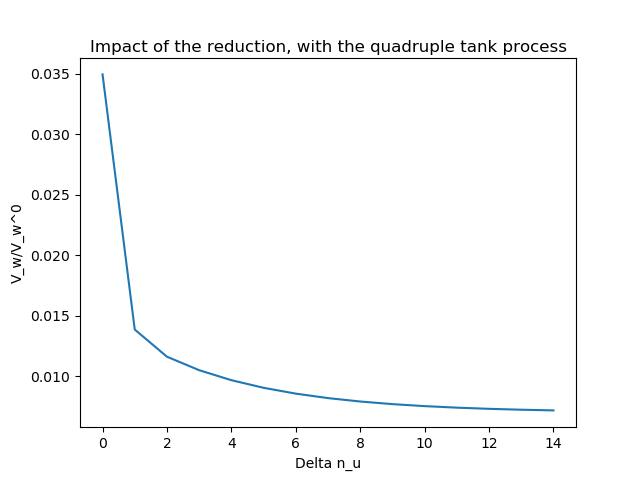
\includegraphics[width=0.9\linewidth]{lin_sys_reduction_seq_control_len}
  \caption{Impact of the variable $\Ninputs$ over the size of the possible state of the reduced system. It does not worth to take $\Ninputs$ greater than 1 since the boundaries of the reduce system does not decrease that much and the complexity of the model exponentially dependant of the number of controls.}
  \label{reduced_system_bounds}
\end{figure}

The next table summaries the gains and loses of this reduction on the previously established criteria.

\begin{tabular}{ l|ll }
& Initial model & Reduced model\\ \hline
Nodes & $\prod_{i=1}^n N_i$ & $\left | U \right |^{\Ninputs} \prod_{i=1}^{n_c} N_i $\\ 
$|U|$ & $n_u$ & $n_u$\\
$V_w$ &  & bigger \\
\end{tabular}

\section{Notes for the future}
Abstractions of asymptotically stable system present a disadvantage on the multiagent control side, for some controls, if the state does not evolve any more, the abstraction will take self loops.
In term multi agent control this make the problem more complex as the control generation: self loops tend to create systems that are asynchronous with all the problems that might occurs because of this (basically one of the agent might be be stopped).

Self loops are not desirable.

Self loops hide any time information (that is why I have been working on the time information chapter).

In the case of the reduction of the abstraction.